\documentclass{article}[12pt]

\usepackage{graphicx}
\usepackage{hyperref}

\title{Geometrysaurus Museum Readme}
\author{Sarah Masters, Mya Longmire, Garrett Bates}

\begin{document}

\maketitle

\section{Repository}

The repository for this project is currently located at: \\

\url{https://github.com/gbbofh/CSE-389-OpenGL-Final-Project}

\section{Changes}

The entire code-base has been mostly rewritten, due to difficulties in
integrating the Open Asset Importer. This new code-base provides two classes,
Mesh and Model, which are used to load and render 3D meshes from WaveFront
Object Files. With this integration, it does away with the WaveFront Loader
which we wrote earlier this semester. This is much to our benefit, as the custom
loader came with a great deal of bugs that would often break the renderer.

These classes provide support for surface normals, UV maps, and vertex
positions; however UV maps are currently not implemented in the shader. That is,
texture mapping is currently not functional. Instead, colour is rendered by
passing the vertex normal to the fragment shader. This has the added effect of
just being kind of pretty.

Additionally, support for lighting has been added -- however the effects are
hard to notice. Currently there exists both ambient lighting, as well as a
single directional light source which is rendered via the fragment shader.

We currently load four models to be rendered:

\begin{description}
        \item[The Room]{Not to be confused with the Tommy Wiseau film of the
                same name -- this room is the museum floorplan, where the user
                can walk around}
        \item[Jerry]{Jerry is a large, friendly tyrannosaurus}
        \item[Randall]{Randy is a tall sauropod. He eats leaves. It's all he does.}
        \item[Bob]{Bob is a parasaurolophus. He Yeets. All. The. Time.
                Nobody likes a Bob.}
\end{description}

We have also included a short video demonstrating the models that have been
loaded, as well as our first person camera.

\section{Images}

Here we have images of the models that we loaded into our application. In
addition to showing them as they were created in Blender 3D, we also include a
brief picture of them being rendered by our application.

\begin{figure}[!ht]
        \centering
        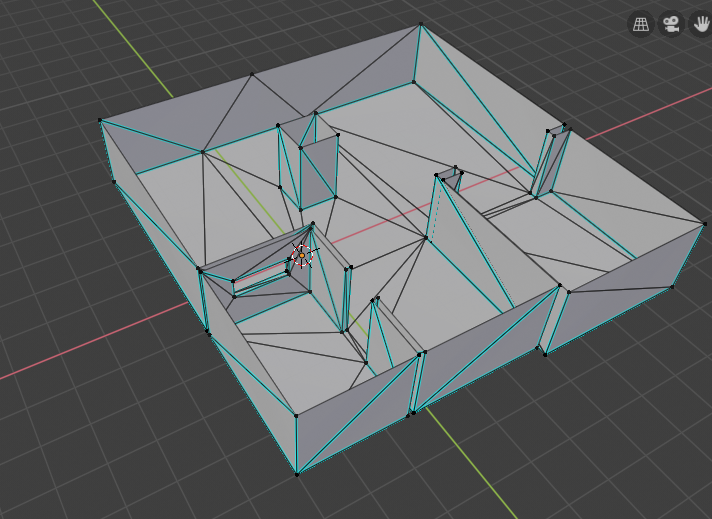
\includegraphics[width=0.8\textwidth]{floorplan.png}
        \caption{The Room}
\end{figure}

\begin{figure}[!ht]
        \centering
        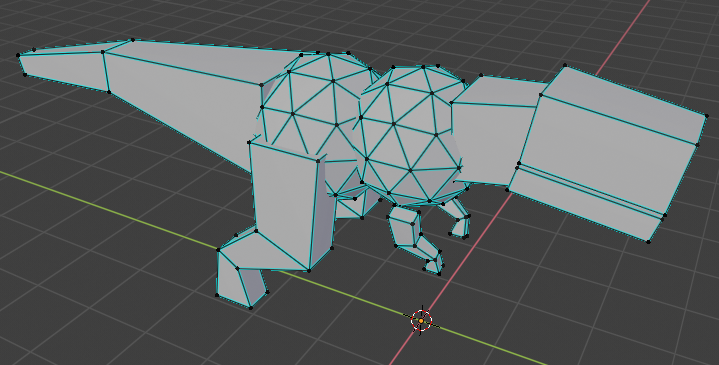
\includegraphics[width=0.8\textwidth]{jerry.png}
        \caption{Jerry}
\end{figure}

\begin{figure}[!ht]
        \centering
        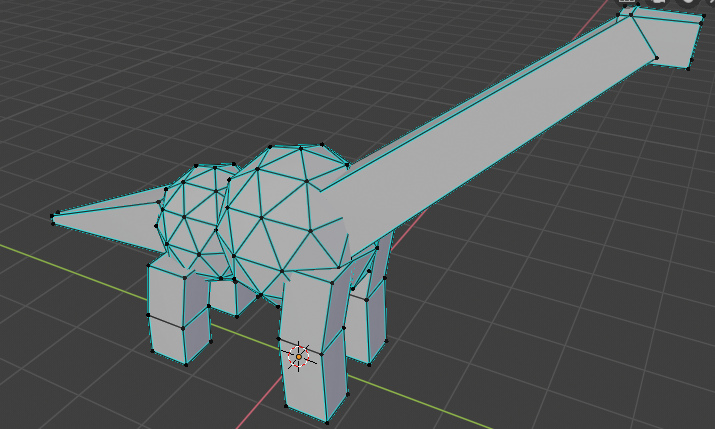
\includegraphics[width=0.8\textwidth]{randall.png}
        \caption{Bob}
\end{figure}

\begin{figure}[!ht]
        \centering
        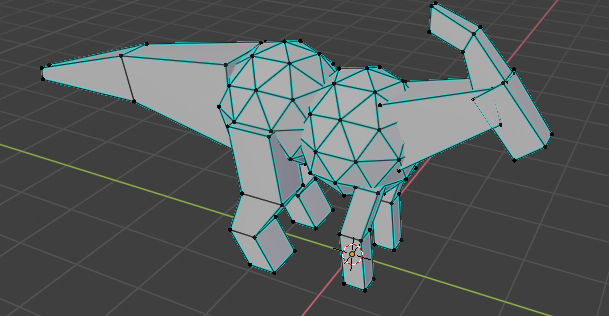
\includegraphics[width=0.8\textwidth]{bob.png}
        \caption{Randall}
\end{figure}

\begin{figure}[!ht]
        \centering
        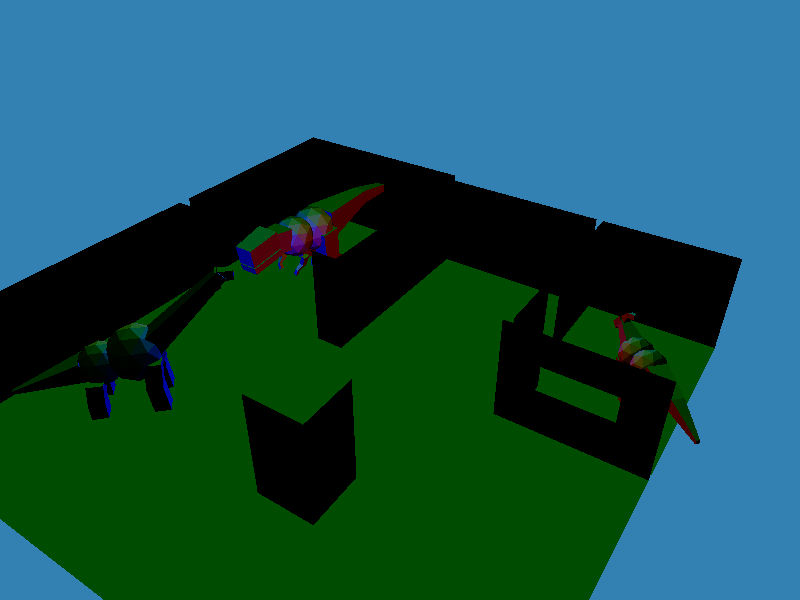
\includegraphics[width=0.8\textwidth]{render.png}
        \caption{Render}
\end{figure}

\end{document}
